% SPDX-FileCopyrightText: 2026 Onur Tuncer and Stereon contributors
% SPDX-License-Identifier: MPL-2.0
%
% This Source Code Form is subject to the terms of the Mozilla Public
% License, v. 2.0. If a copy of the MPL was not distributed with this
% file, You can obtain one at https://mozilla.org/MPL/2.0/.
%
% ADR-0001's merge policy (docs/tolerances.rst). Four vertices in a chain,
% each 0.8 tau from the next: proximity is not transitive. Processed in
% order, A opens a cluster as its representative; B lies within tau of A
% and joins; C lies within tau of B but 1.6 tau from A, the representative,
% so it opens a cluster of its own, which D joins. Single linkage would
% have merged all four, a cluster 2.4 tau wide.
\documentclass[tikz,border=6pt]{standalone}
\usetikzlibrary{arrows.meta,decorations.pathreplacing}
\definecolor{one}{RGB}{31,119,180}
\definecolor{two}{RGB}{255,127,14}
\begin{document}
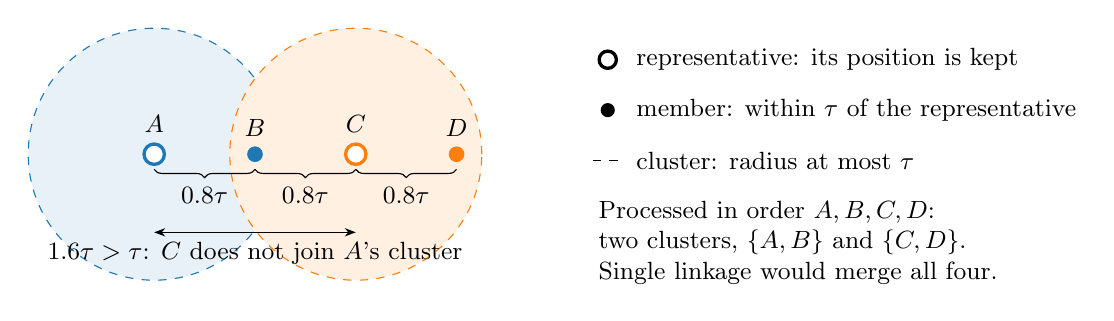
\begin{tikzpicture}[scale=1.6,lbl/.style={font=\small},
    rep/.style={circle,draw,very thick,inner sep=2.6pt},
    mem/.style={circle,fill,inner sep=2pt}]
  \def\tol{1}
  % Clusters: a disc of radius tau about each representative
  \fill[one!10] (0,0) circle (\tol);
  \draw[one,dashed] (0,0) circle (\tol);
  \fill[two!12] (1.6,0) circle (\tol);
  \draw[two,dashed] (1.6,0) circle (\tol);
  % The four vertices
  \node[rep,draw=one,fill=white,label={[lbl]above:$A$}] (A) at (0,0) {};
  \node[mem,one,label={[lbl]above:$B$}] (B) at (0.8,0) {};
  \node[rep,draw=two,fill=white,label={[lbl]above:$C$}] (C) at (1.6,0) {};
  \node[mem,two,label={[lbl]above:$D$}] (D) at (2.4,0) {};
  % Spacings
  \foreach \x/\y in {0/0.8,0.8/1.6,1.6/2.4}
    \draw[decorate,decoration={brace,amplitude=3pt,mirror}] (\x,-0.12) -- (\y,-0.12)
      node[lbl,midway,below=3pt] {$0.8\tau$};
  \draw[{Stealth[length=4pt]}-{Stealth[length=4pt]}] (0,-0.62) -- (1.6,-0.62)
      node[lbl,midway,below] {$1.6\tau > \tau$: $C$ does not join $A$'s cluster};
  % Legend
  \begin{scope}[shift={(3.6,0.75)},lbl]
    \node[rep,draw=black,fill=white,inner sep=2.2pt] at (0,0) {};
    \node[right] at (0.15,0) {representative: its position is kept};
    \node[mem,inner sep=1.8pt] at (0,-0.4) {};
    \node[right] at (0.15,-0.4) {member: within $\tau$ of the representative};
    \draw[dashed] (-0.12,-0.8) -- (0.12,-0.8);
    \node[right] at (0.15,-0.8) {cluster: radius at most $\tau$};
    \node[right,align=left] at (-0.15,-1.45) {Processed in order $A, B, C, D$:\\
      two clusters, $\{A,B\}$ and $\{C,D\}$.\\
      Single linkage would merge all four.};
  \end{scope}
\end{tikzpicture}
\end{document}
